\subsection{\label{sec:calib.dc}Drift Chambers}

\subsubsection{\label{sec:DC.TOF.res}Drift Chamber and TOF smearing parameters in \prog{gpp}}

Tracking in the Drift Chamber of a \abbr{CLAS} Sector is performed using the six superlayers of the \abbr{DC}. A good measure of the the quality of tracking are the \abbr{DC} residuals for each superlayer. After a track is identified using the hit elements in the \abbr{DC} superlayer, It's \abbr{DC} residual is calculated using the TBLA bank as follows:

\begin{verbatim}
fabs(TBLA->tbla[i].fitdoca) - fabs(TBLA->tbla[i].calcdoca)
\end{verbatim}

The values of the DC residuals in the CLAS data are empirically found to be a good fit to a convolution of 2 gaussians - a narrow gaussian and a broad gaussian. During DC calibrations efforts were made to minimise this residual to have maximum reconstruction efficiency. As stated earlier, the goal of using GPP is to simulate the experimental conditions as close as possible. So we smear the values of the DOCA for the simulated tracks with a single gaussian whose width is equal to the events weighted sum of the widths of the two gaussians fitted to the data from the run 56855. This makes the residual for a superlayer in the simulated data approximately equal to the weighted residual from the real data. The default available options for GPP specifies only three parameters `-a, -b, -c' for DC DOCA smearing, where each parameter is responsible for the smearing of two superlayers (in one Region) of all six sectors. Hence, we choose a set of parameters based on the following fits as seen in Figs.~\ref{fig:SLRes} and \ref{fig:SLRes_default}, which gives us the best match on average between the different superlayers in the six sectors (see Fig.~\ref{fig:DC_SL_Match}).

\begin{figure}[htpb]\begin{center}
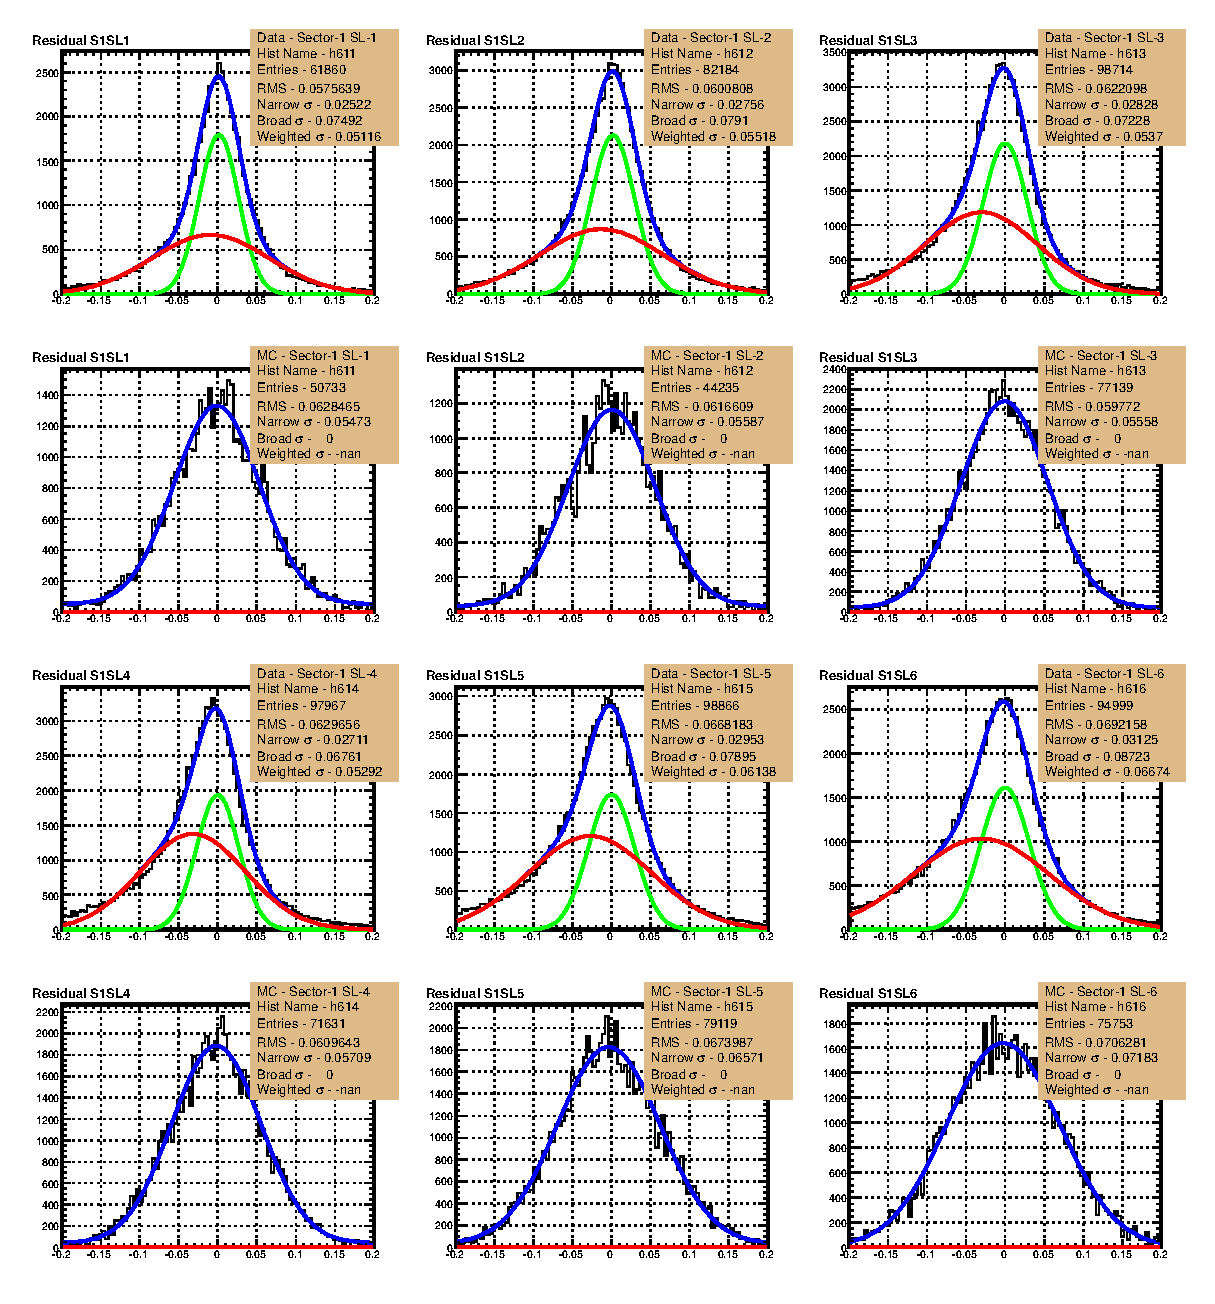
\includegraphics[width=0.8\columnwidth]{figures/calib/dc/Sector_1_compare.eps}
\caption[DC superlayers Resolution Matching]{\label{fig:SLRes}Plots and Fits used to match the residuals (resolution) for Drift Chamber superlayers in CLAS Sector 1, between the Data and the Simulation. Data is an empirical fit to a convolution of two gaussians. The simulated distribution is a single gaussian with its simulated width approximately equal to the weighed sum of the widths of the two gaussians fitted to the data. This simulation uses the best estimated smearing parameters to match the DC residuals, between the Data and the Simulation.}
\end{center}\end{figure}

\begin{figure}[htpb]\begin{center}
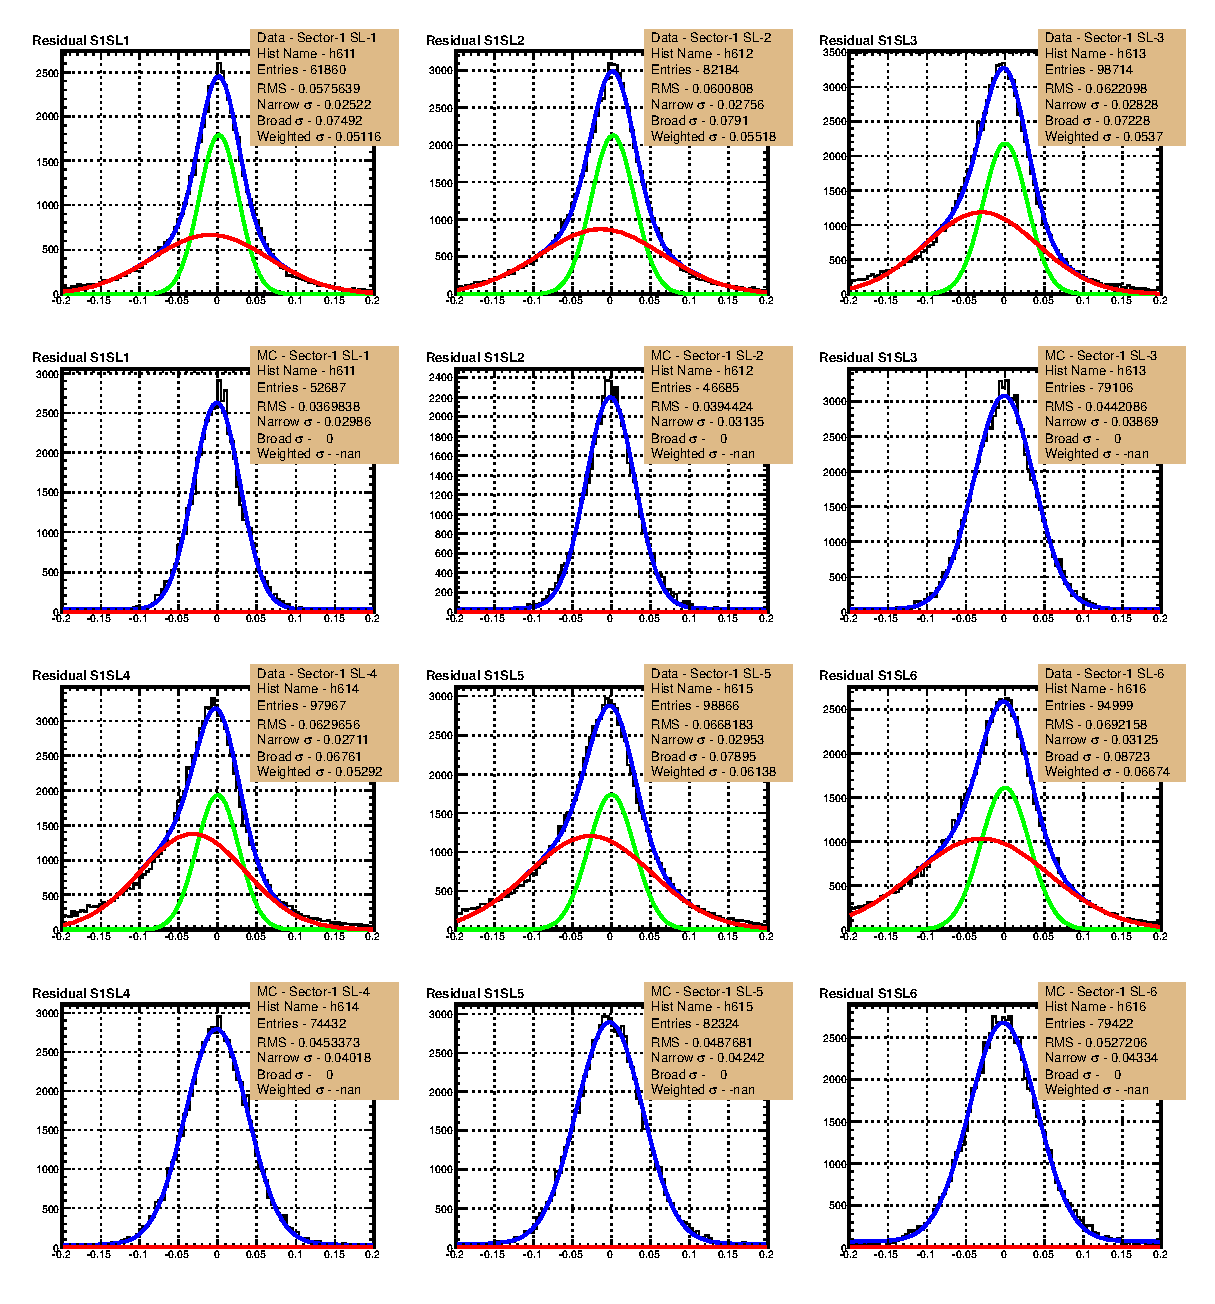
\includegraphics[width=\columnwidth]{figures/calib/dc/Sector_1_compare_default.eps}
\caption[DC superlayers Resolution Matching]{\label{fig:SLRes_default}Plots and Fits used to compare the residuals (resolution) for Drift Chamber superlayers in CLAS Sector 1, between the Data and the Simulation using the default GPP smearing.}
\end{center}\end{figure}

\begin{figure}[htpb]\begin{center}
\subfigure{
    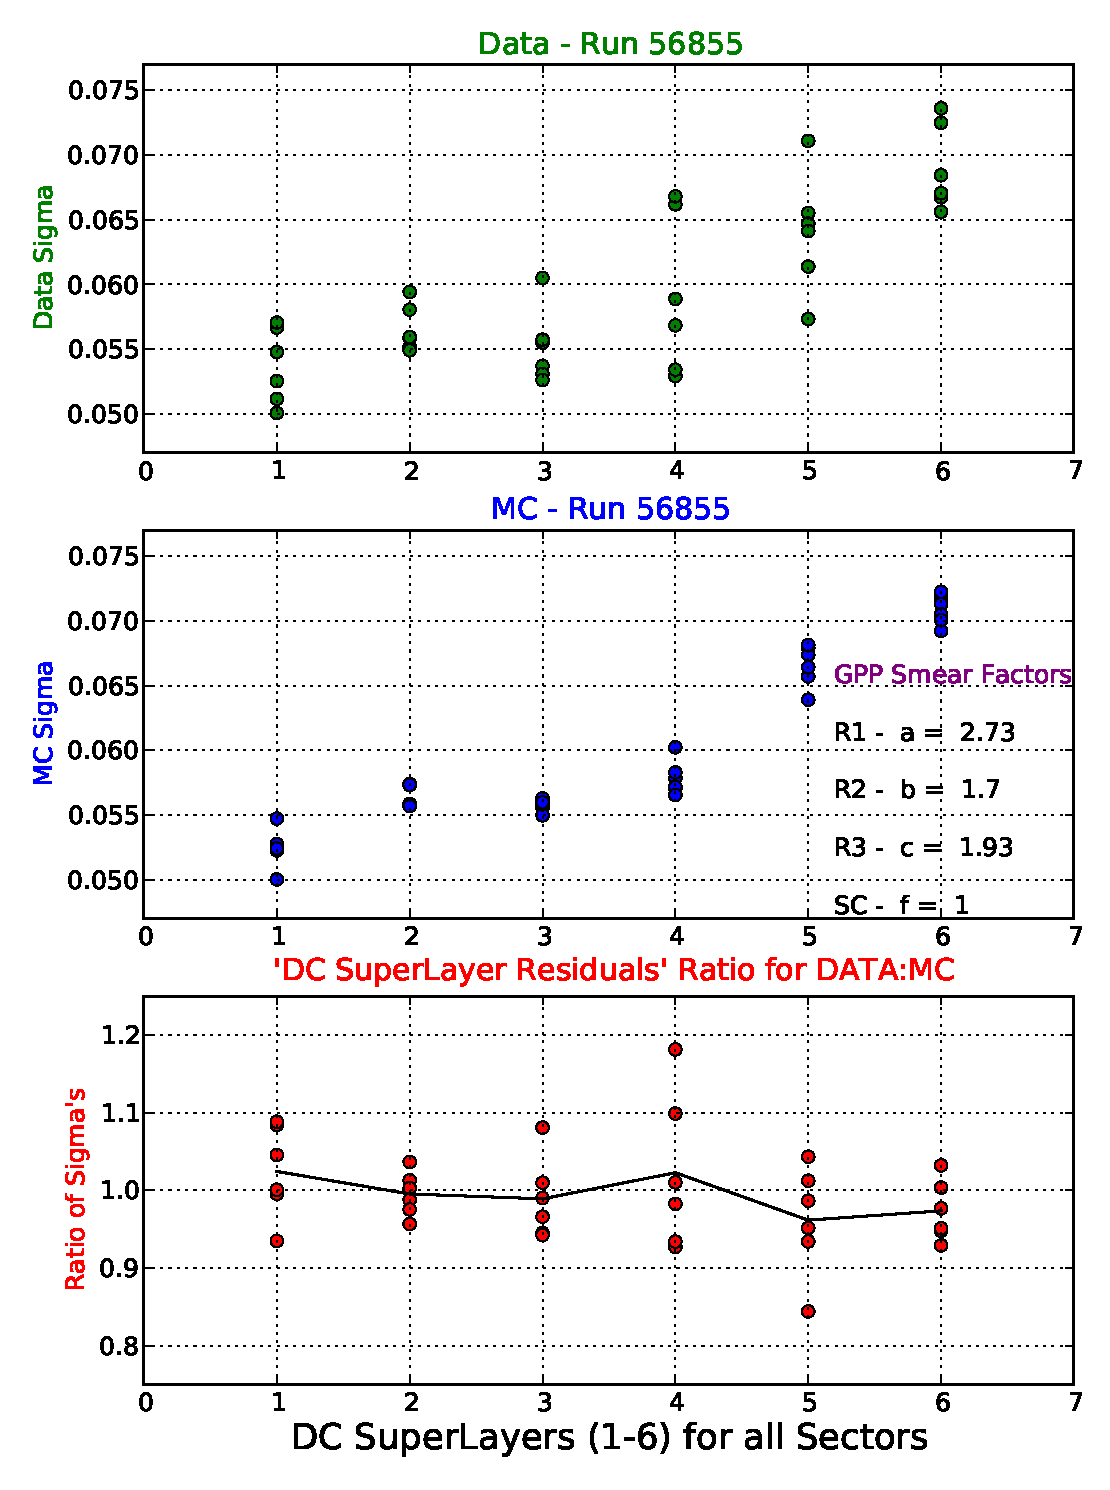
\includegraphics[width=0.47\columnwidth]{figures/calib/dc/DC_Sigma_SL.eps}
    \label{fig:DC_SL_best}
}
\subfigure{
    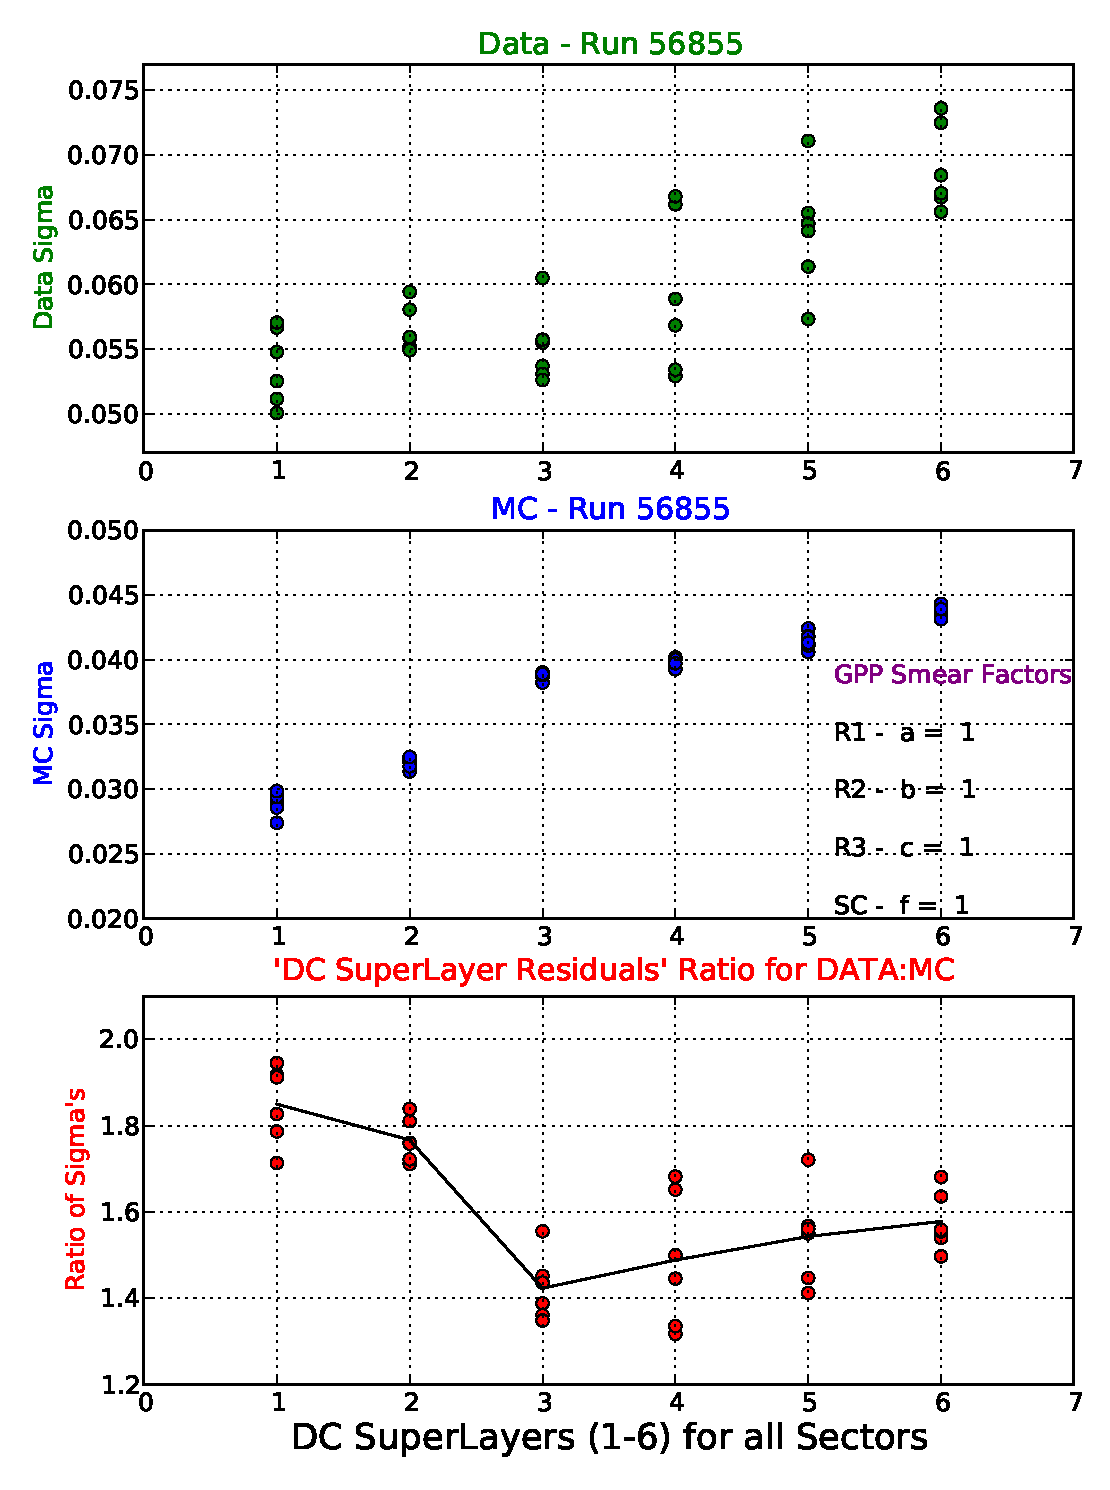
\includegraphics[width=0.47\columnwidth]{figures/calib/dc/DC_Sigma_SL_default.eps}
    \label{fig:DC_SL_default}
}
\caption[DC superlayers Resolution Matching]{\label{fig:DC_SL_Match}Comparison of the DC residuals on a superlayer basis for all the CLAS sectors for real as well as simulated events. The left plots use the best estimated smearing parameters for the DC DOCA to match the real and simulated data shown in Figure~\ref{fig:SLRes}., whereas the right plots use the default GPP smearing shown in Figure~\ref{fig:SLRes_default}.}
\end{center}\end{figure}

The smearing parameter `-f' for the Time of Flight timing resolution is one of the GPP parameters that is usually used to match the quality of data and simulation. Using the reference run 56855, we observe that the default GPP smearing is adequate (see Figure \ref{fig:TOF_Res}).

\begin{figure}[htpb]\begin{center}
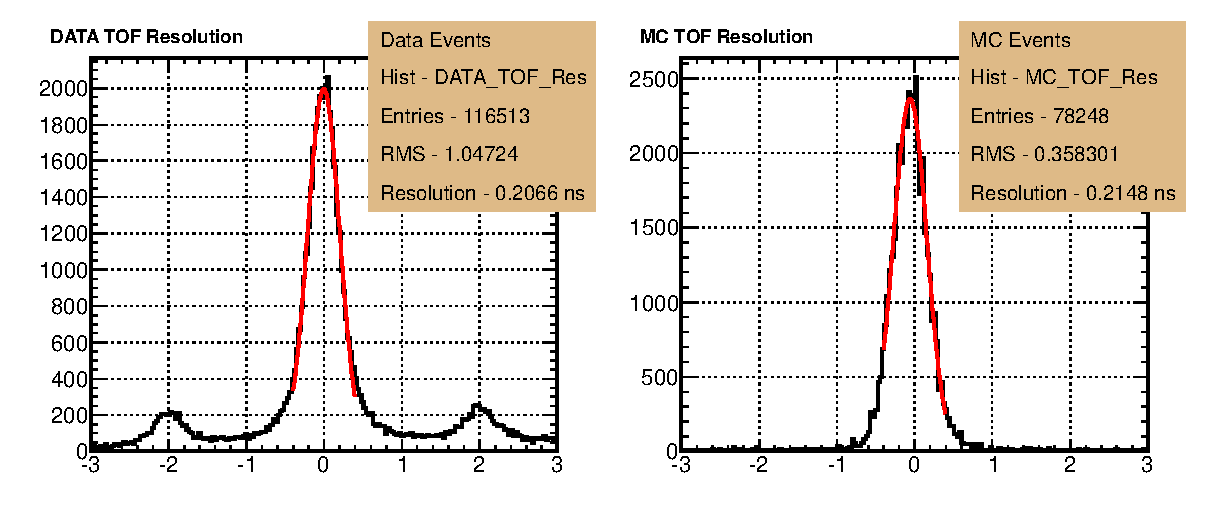
\includegraphics[width=\columnwidth]{figures/calib/dc/TOF_Compare.eps}
\caption[TOF Resolution Matching]{\label{fig:TOF_Res}Plots and Fits used to match the TOF timing resolution. The default smearing of GPP was found to be adequate in this case.}
\end{center}\end{figure}

These smearing parameters affect the reconstruction efficiency for the tracks in CLAS during simulations. A rudimentary analysis quantifying the effect is presented in Table~\ref{tab:recon.eff}. As expected, as the Drift chamber response becomes more noisy due to smearing of DOCA (higher DC residuals), the reconstruction and tracking efficiency in CLAS goes down.

\begin{table}
\begin{center}
\begin{minipage}{\textwidth}
\caption{\label{tab:recon.eff} Measure of Track Reconstruction Efficiency for sets of \texttt{gpp} parameters}
\begin{center}
\begin{tabular}{cccc}
\hline \hline
Generated  &  Accepted  & Reconstruction Acceptance & \texttt{gpp} Smearing Factors (a, b, c, f)\\
\hline
90000 & 1217 & 1.352\% & R1=1, R2=1, R3=1, SC=1\\
90000 & 1161 & 1.29\%  & R1=2.73, R2=1.7, R3=1.93, SC=1\\
90000 & 1053 & 1.17\%  & R1=2.73, R2=1.7, R3=1.93, SC=2 \\
\hline \hline
\end{tabular}
\end{center}
\end{minipage}
\end{center}
\end{table}

\FloatBarrier
